% Options for packages loaded elsewhere
\PassOptionsToPackage{unicode}{hyperref}
\PassOptionsToPackage{hyphens}{url}
%
\documentclass[
  12pt,
]{article}
\usepackage{amsmath,amssymb}
\usepackage{iftex}
\ifPDFTeX
  \usepackage[T1]{fontenc}
  \usepackage[utf8]{inputenc}
  \usepackage{textcomp} % provide euro and other symbols
\else % if luatex or xetex
  \usepackage{unicode-math} % this also loads fontspec
  \defaultfontfeatures{Scale=MatchLowercase}
  \defaultfontfeatures[\rmfamily]{Ligatures=TeX,Scale=1}
\fi
\usepackage{lmodern}
\ifPDFTeX\else
  % xetex/luatex font selection
\fi
% Use upquote if available, for straight quotes in verbatim environments
\IfFileExists{upquote.sty}{\usepackage{upquote}}{}
\IfFileExists{microtype.sty}{% use microtype if available
  \usepackage[]{microtype}
  \UseMicrotypeSet[protrusion]{basicmath} % disable protrusion for tt fonts
}{}
\makeatletter
\@ifundefined{KOMAClassName}{% if non-KOMA class
  \IfFileExists{parskip.sty}{%
    \usepackage{parskip}
  }{% else
    \setlength{\parindent}{0pt}
    \setlength{\parskip}{6pt plus 2pt minus 1pt}}
}{% if KOMA class
  \KOMAoptions{parskip=half}}
\makeatother
\usepackage{xcolor}
\usepackage[margin=1in]{geometry}
\usepackage{color}
\usepackage{fancyvrb}
\newcommand{\VerbBar}{|}
\newcommand{\VERB}{\Verb[commandchars=\\\{\}]}
\DefineVerbatimEnvironment{Highlighting}{Verbatim}{commandchars=\\\{\}}
% Add ',fontsize=\small' for more characters per line
\usepackage{framed}
\definecolor{shadecolor}{RGB}{248,248,248}
\newenvironment{Shaded}{\begin{snugshade}}{\end{snugshade}}
\newcommand{\AlertTok}[1]{\textcolor[rgb]{0.94,0.16,0.16}{#1}}
\newcommand{\AnnotationTok}[1]{\textcolor[rgb]{0.56,0.35,0.01}{\textbf{\textit{#1}}}}
\newcommand{\AttributeTok}[1]{\textcolor[rgb]{0.13,0.29,0.53}{#1}}
\newcommand{\BaseNTok}[1]{\textcolor[rgb]{0.00,0.00,0.81}{#1}}
\newcommand{\BuiltInTok}[1]{#1}
\newcommand{\CharTok}[1]{\textcolor[rgb]{0.31,0.60,0.02}{#1}}
\newcommand{\CommentTok}[1]{\textcolor[rgb]{0.56,0.35,0.01}{\textit{#1}}}
\newcommand{\CommentVarTok}[1]{\textcolor[rgb]{0.56,0.35,0.01}{\textbf{\textit{#1}}}}
\newcommand{\ConstantTok}[1]{\textcolor[rgb]{0.56,0.35,0.01}{#1}}
\newcommand{\ControlFlowTok}[1]{\textcolor[rgb]{0.13,0.29,0.53}{\textbf{#1}}}
\newcommand{\DataTypeTok}[1]{\textcolor[rgb]{0.13,0.29,0.53}{#1}}
\newcommand{\DecValTok}[1]{\textcolor[rgb]{0.00,0.00,0.81}{#1}}
\newcommand{\DocumentationTok}[1]{\textcolor[rgb]{0.56,0.35,0.01}{\textbf{\textit{#1}}}}
\newcommand{\ErrorTok}[1]{\textcolor[rgb]{0.64,0.00,0.00}{\textbf{#1}}}
\newcommand{\ExtensionTok}[1]{#1}
\newcommand{\FloatTok}[1]{\textcolor[rgb]{0.00,0.00,0.81}{#1}}
\newcommand{\FunctionTok}[1]{\textcolor[rgb]{0.13,0.29,0.53}{\textbf{#1}}}
\newcommand{\ImportTok}[1]{#1}
\newcommand{\InformationTok}[1]{\textcolor[rgb]{0.56,0.35,0.01}{\textbf{\textit{#1}}}}
\newcommand{\KeywordTok}[1]{\textcolor[rgb]{0.13,0.29,0.53}{\textbf{#1}}}
\newcommand{\NormalTok}[1]{#1}
\newcommand{\OperatorTok}[1]{\textcolor[rgb]{0.81,0.36,0.00}{\textbf{#1}}}
\newcommand{\OtherTok}[1]{\textcolor[rgb]{0.56,0.35,0.01}{#1}}
\newcommand{\PreprocessorTok}[1]{\textcolor[rgb]{0.56,0.35,0.01}{\textit{#1}}}
\newcommand{\RegionMarkerTok}[1]{#1}
\newcommand{\SpecialCharTok}[1]{\textcolor[rgb]{0.81,0.36,0.00}{\textbf{#1}}}
\newcommand{\SpecialStringTok}[1]{\textcolor[rgb]{0.31,0.60,0.02}{#1}}
\newcommand{\StringTok}[1]{\textcolor[rgb]{0.31,0.60,0.02}{#1}}
\newcommand{\VariableTok}[1]{\textcolor[rgb]{0.00,0.00,0.00}{#1}}
\newcommand{\VerbatimStringTok}[1]{\textcolor[rgb]{0.31,0.60,0.02}{#1}}
\newcommand{\WarningTok}[1]{\textcolor[rgb]{0.56,0.35,0.01}{\textbf{\textit{#1}}}}
\usepackage{graphicx}
\makeatletter
\def\maxwidth{\ifdim\Gin@nat@width>\linewidth\linewidth\else\Gin@nat@width\fi}
\def\maxheight{\ifdim\Gin@nat@height>\textheight\textheight\else\Gin@nat@height\fi}
\makeatother
% Scale images if necessary, so that they will not overflow the page
% margins by default, and it is still possible to overwrite the defaults
% using explicit options in \includegraphics[width, height, ...]{}
\setkeys{Gin}{width=\maxwidth,height=\maxheight,keepaspectratio}
% Set default figure placement to htbp
\makeatletter
\def\fps@figure{htbp}
\makeatother
\setlength{\emergencystretch}{3em} % prevent overfull lines
\providecommand{\tightlist}{%
  \setlength{\itemsep}{0pt}\setlength{\parskip}{0pt}}
\setcounter{secnumdepth}{-\maxdimen} % remove section numbering
\usepackage{titlesec}
\usepackage{setspace}
\newcommand{\sectionbreak}{\clearpage}
\usepackage{fontspec}
\setmainfont{Times New Roman}
\ifLuaTeX
  \usepackage{selnolig}  % disable illegal ligatures
\fi
\usepackage{bookmark}
\IfFileExists{xurl.sty}{\usepackage{xurl}}{} % add URL line breaks if available
\urlstyle{same}
\hypersetup{
  pdfauthor={Anna Movsisyan; Ani Aloyan; Elina Ohanjanyan; Lusine Aghinyan},
  hidelinks,
  pdfcreator={LaTeX via pandoc}}

\title{Exploring AUA's Student Performance}
\usepackage{etoolbox}
\makeatletter
\providecommand{\subtitle}[1]{% add subtitle to \maketitle
  \apptocmd{\@title}{\par {\large #1 \par}}{}{}
}
\makeatother
\subtitle{IESM315 Design Analysis and Experiment - Final Project\\
Instructor: Tadamasa Sawada}
\author{Anna Movsisyan \and Ani Aloyan \and Elina Ohanjanyan \and Lusine
Aghinyan}
\date{10 December, 2024}

\begin{document}
\maketitle

{
\setcounter{tocdepth}{2}
\tableofcontents
}
\doublespacing

\newpage

\section{Abstract}\label{abstract}

This report aims to analyze the American University of Armenia (AUA)
student GPA statistics provided by AUA's Office of Institutional
Research and Assessment (OIRA). The study identifies patterns in
academic performance across metrics such as colleges, majors, genders,
financial aid satus, etc. This analysis highlights trends and potential
factors that affect the final cumulative GPA of students.

\section{Data Collection}\label{data-collection}

The data for this study was obtained from AUA's OIRA. Key variables
included:

\begin{itemize}
\tightlist
\item
  \textbf{Student ID}: Numeric code assigned to students.
\item
  \textbf{FirstEnrolled\_MajorCode}: Initial major of enrollment.
\item
  \textbf{College}: College associated with each major.
\item
  \textbf{FincialAid\_Received\_AtLeast\_Once}: Binary variable
  indicating whether financial aid was received.
\item
  \textbf{FirstEnrolled\_Year}: Year of initial enrollment.
\item
  \textbf{Gender}: Gender information of students.
\item
  \textbf{School\_GPA}: Standardized GPA (0-5 scale).
\item
  \textbf{RoA (Republic of Armenia)}: Binary variable indicating
  citizenship.
\item
  \textbf{FirstYear\_CGPA}: GPA for the first year.
\item
  \textbf{All\_CGPA}: Cumulative GPA.
\end{itemize}

Data privacy concerns led to the exclusion of rows with a count of five
or fewer to ensure student anonymity.

\section{A Glance at the Data}\label{a-glance-at-the-data}

\begin{verbatim}
## # A tibble: 2,706 x 10
##    Studen~1 First~2 College Finci~3 First~4 Gender Schoo~5   RoA First~6 All_C~7
##       <dbl> <chr>   <chr>     <dbl>   <dbl> <chr>    <dbl> <dbl>   <dbl>   <dbl>
##  1  6.27e 9 BAB     CBE           0    2014 Male      3.81     1   0.189   0.189
##  2  4.18e 9 BAB     CBE           0    2018 Male      4.12     1  NA      NA    
##  3  4.69e 9 BSCS    CSE           0    2013 Male      4        1   0.856   0.856
##  4  4.22e 9 BAB     CBE           0    2015 Male      3.56     1   2.25    2.75 
##  5  1.50e10 BAB     CBE           0    2015 Male      3.9      1   2.3     1.52 
##  6  8.18e 9 BSCS    CSE           0    2015 Male      4.00     1  NA      NA    
##  7  6.52e 9 BSCS    CSE           0    2019 Male      4.18     1   2.15   NA    
##  8  1.56e10 BAB     CBE           1    2016 Male      4.18     1  NA      NA    
##  9  6.08e 9 BAB     CBE           1    2017 Male      4        1   3.87   NA    
## 10  1.27e10 BAB     CBE           0    2020 Male      4.44     0   3.13   NA    
## # ... with 2,696 more rows, and abbreviated variable names 1: `Student ID`,
## #   2: FirstEnrolled_MajorCode, 3: FincialAid_Received_AtLeast_Once,
## #   4: FirstEnrolled_Year, 5: School_GPA, 6: FirstYear_CGPA, 7: All_CGPA
\end{verbatim}

\newpage

\begin{figure}
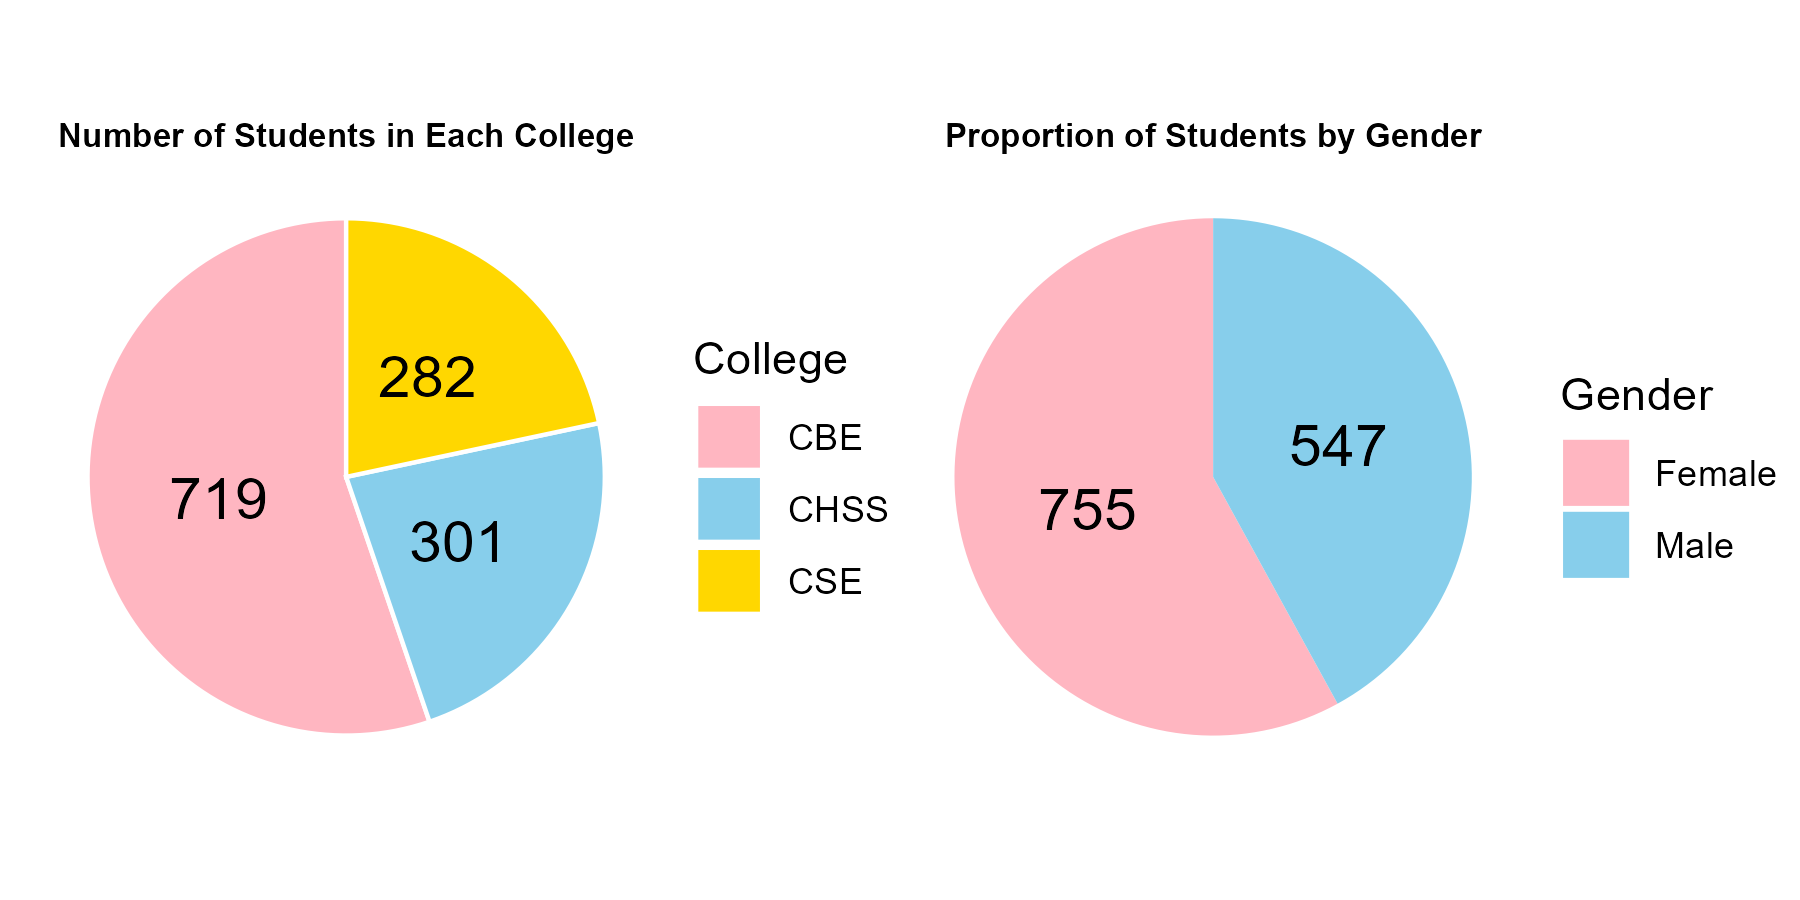
\includegraphics[width=0.8\linewidth]{combined_plot} \caption{Distribution of AUA Students by College and Gender}\label{fig:unnamed-chunk-5}
\end{figure}

The piecharts show the distribution of students by 1) College and 2)
Gender.

As it can be seen from Fig. 1, the College of CSE has the most number of
enrolled students, CHSS and CSE are relatively closer to each other in
numbers and more than twice as less than CBE. Looking at the
distribution by gender, it is seen that the number of female students
exceeds the number of male students by \textasciitilde200.

\begin{figure}
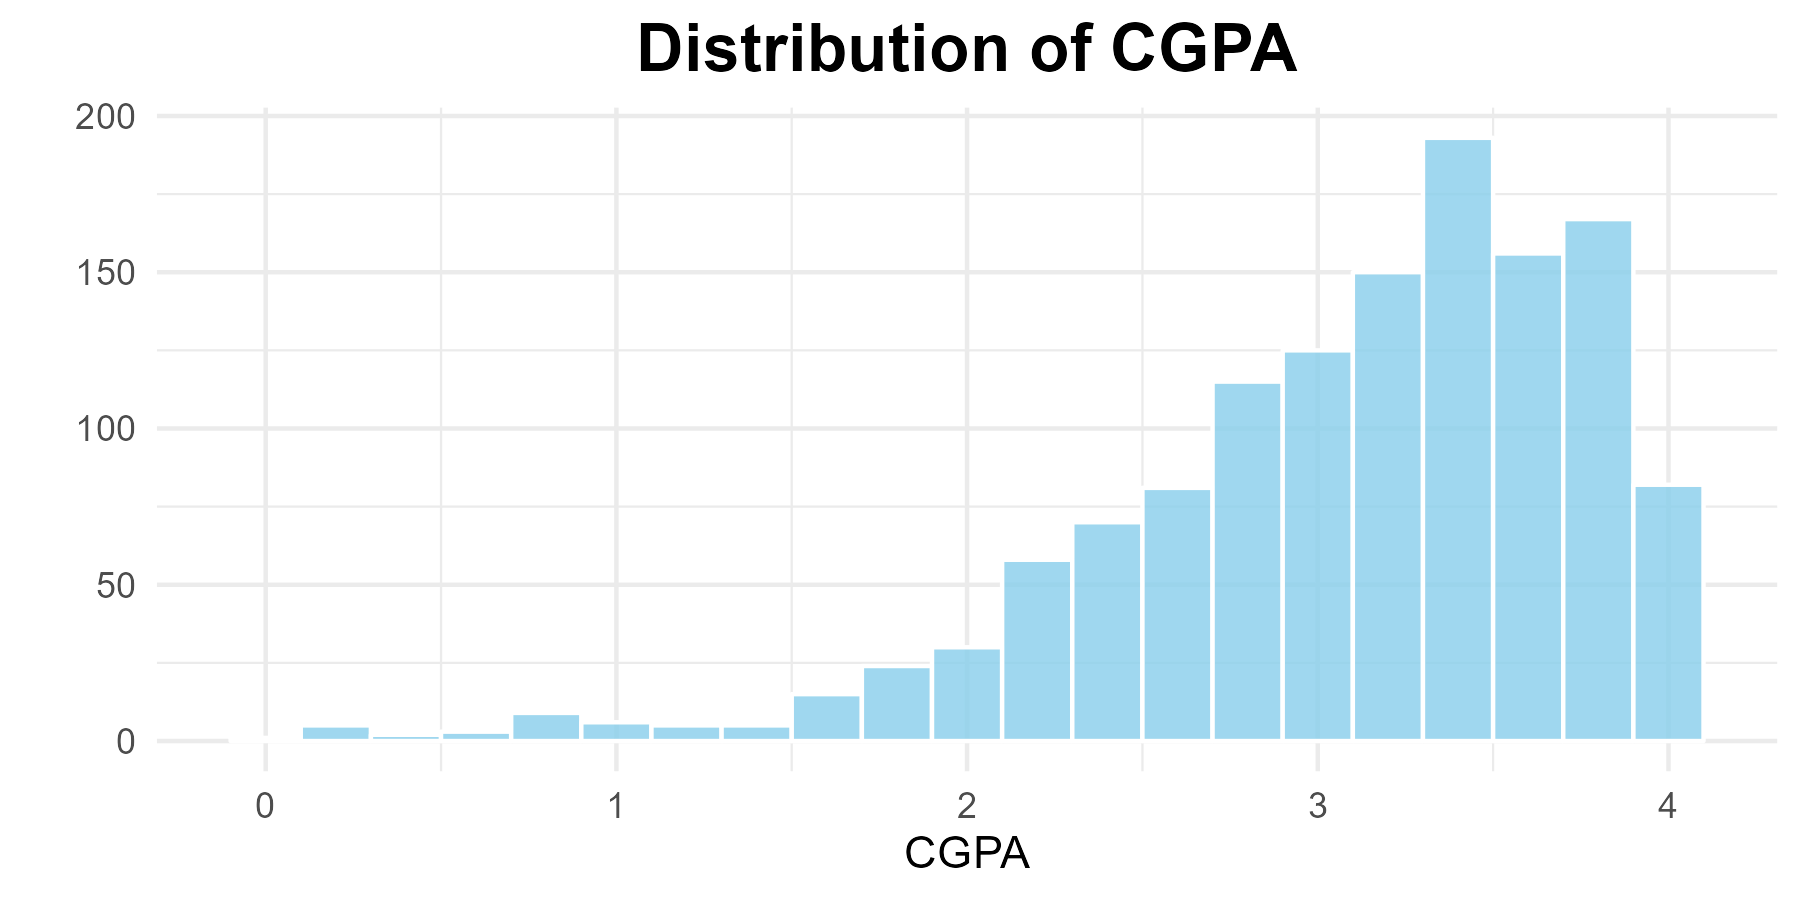
\includegraphics[width=0.8\linewidth]{histogram} \caption{Histogram of CGPA}\label{fig:unnamed-chunk-6}
\end{figure}

Now a glance at the distribution of All Cumulative GPA from Fig. 2. From
the plot, it can be seen that the distribution is skewed and has a
concentration around 3.3-3.7.

\section{Literature Review}\label{literature-review}

To better understand the effects of some of our factors on students'
performances, we conducted a Literature Review and studued some articles
that tested some similr factors.

\subsection{Factors Influencing College Persistence for First-Time
Students}\label{factors-influencing-college-persistence-for-first-time-students}

The first article chosen to study the influce of the factors present in
our dataset was article''Factors Influencing College Persistence for
First-Time Students'' by Sheilynda Stewart, Doo Hun Lim, and JoHyun Kim.
It examines various factors that impact whether students persist in
their college education (which, admittedly, is different from studying
the influence of these factors on the students' GPA). Some of the key
points we want to highlight are:

\begin{itemize}
\item
  \textbf{Need-Based Grants:} The authors highlight the positive role of
  financial aid, particularly need-based grants (which is similar to the
  Financial Aid granted to the students by AUA), in supporting college
  persistence. These grants reduce financial stress and help students
  from lower socioeconomic backgrounds stay enrolled, demonstrating
  their significant influence on retention rates.
\item
  \textbf{Gender:} Findings on gender differences in persistence are
  mixed. Some studies cited in the article reveal that women persist and
  graduate at higher rates compared to men, while others show no
  significant gender differences in dropout behavior. The resulrs of the
  study itself did not indicate that gender is significant when it comes
  to college persistence. This indicates that gender may interact with
  other factors, such as major or institutional characteristics, to
  influence outcomes.
\item
  \textbf{School GPA:} According to this study, academic performance, as
  reflected in a student's High School and First Year College GPA, is a
  strong predictor of persistence. Students with higher GPAs are more
  likely to stay enrolled and complete their degrees. A strong academic
  foundation during the first year appears critical in sustaining
  momentum toward graduation. However, it is import to take into
  consideration the fact that the high school GPAs of the students used
  in this study were self-reported, so the findings may have some
  inaccuracies.
\end{itemize}

\subsection{Collegeboard Analysis}\label{collegeboard-analysis}

The second source chosen for understanding our factor is the was an
analysis conducted by Collegeboard (the organization responsible for
conducting the SAT tests) called ``Using SAT Scores to Inform Academic
Major-Related Decisions and Planning on Campus'' by Paul A. Westrick,
Jessica P. Marini, and Emily J. Shaw. While the overall goal of the
study was not the analysis of college performance, it did include some
interesting findings that may be useful to us in the future.

The most interesting finding for our study was the following plot:

\begin{figure}
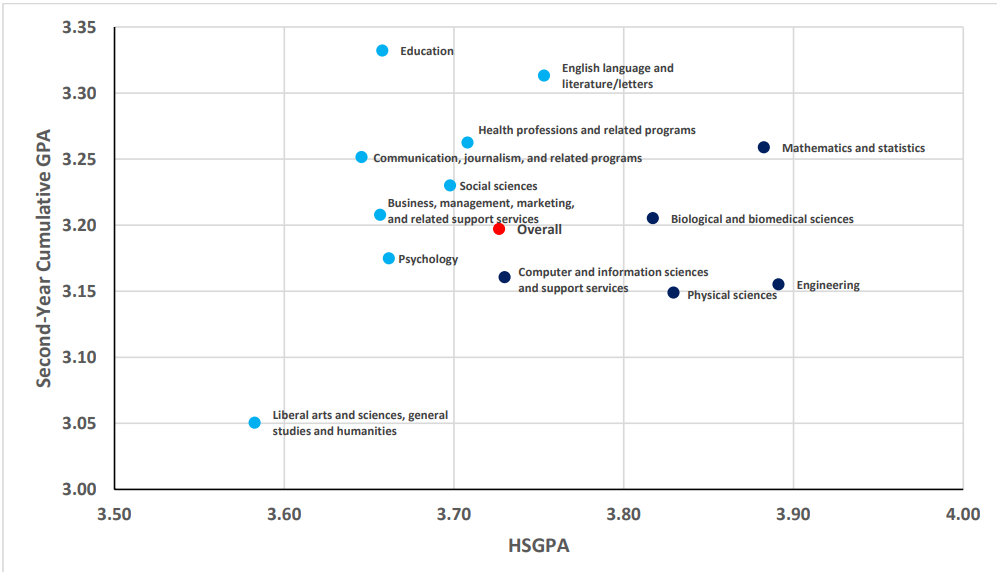
\includegraphics[width=0.95\linewidth]{collegeboard} \caption{Relationship Between High School and College GPA by Major}\label{fig:unnamed-chunk-7}
\end{figure}

As can be seen in Fig. 3, the reason why we wanted to focus on this
study is because it shows some interesting trends about how the major of
the students can correlate with their High School and College GPA. Some
of the interesting points that can be derived from this plot are: -
\textbf{Science Majors:} One of the more interesting things on this plot
is the fact that while Science majors (Math, Engineering, etc) have the
highest GPAs in their school years, their College GPAs seem to be
somewhat lower than that of the other majors in college. -
\textbf{Business Majors:} Another interesting statistic is that Business
majors are around the middle in both high school and college GPA. -
\textbf{Communications Majors:} The last finding that can be somewhat
related to our data is the fact Communications majors (which can
correspond to the students in AUA's English and Communications program),
despite having a relatively lower High School GPA, have one of the
highest GPAs in College.

However, it is important to note that the study was conducted on the
data of US students and might not reflect some trends present in the
Armenian education system.

\subsection{Ethnic and gender stereotypes on college students' academic
performance}\label{ethnic-and-gender-stereotypes-on-college-students-academic-performance}

The last article we will discuss is Ethnic and gender stereotypes on
college students' academic performance'' by Ya-Wen (Melissa) Liang, Don
Jones and Rebecca A. Robles-Pina. The reason why this article can be
somewhat relevant is because it was conducted at a small university in
Texas. While this does not directly correlate to Armenia, it is still
important to note that Texas, being one of the more conservative states
in the U.S., can show somewhat similar soicietal factors to Armenia, a
very conservative country.

The main finding of this study was that gender had a significant effect
on the students'GPA, and female students had a higher GPA than males.

\section{Exploratory Data Analysis
(EDA)}\label{exploratory-data-analysis-eda}

\begin{figure}
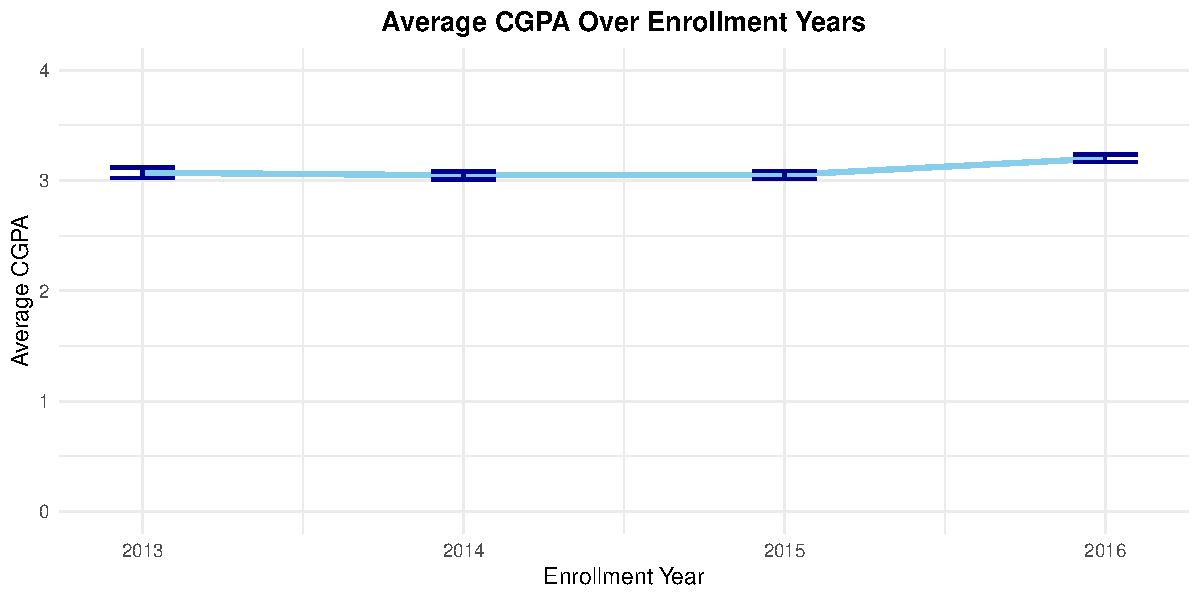
\includegraphics[width=0.9\linewidth]{iesm315_report_files/figure-latex/unnamed-chunk-8-1} \caption{Average CGPA by Cohort}\label{fig:unnamed-chunk-8}
\end{figure}

Fig. 4 shows the average CGPA (with error bar by standard error) over
the enrollment years. As it can be observed, there is almost no
difference between the cohorts of different years and their average is
slightly higher tha 3.0.

\begin{figure}
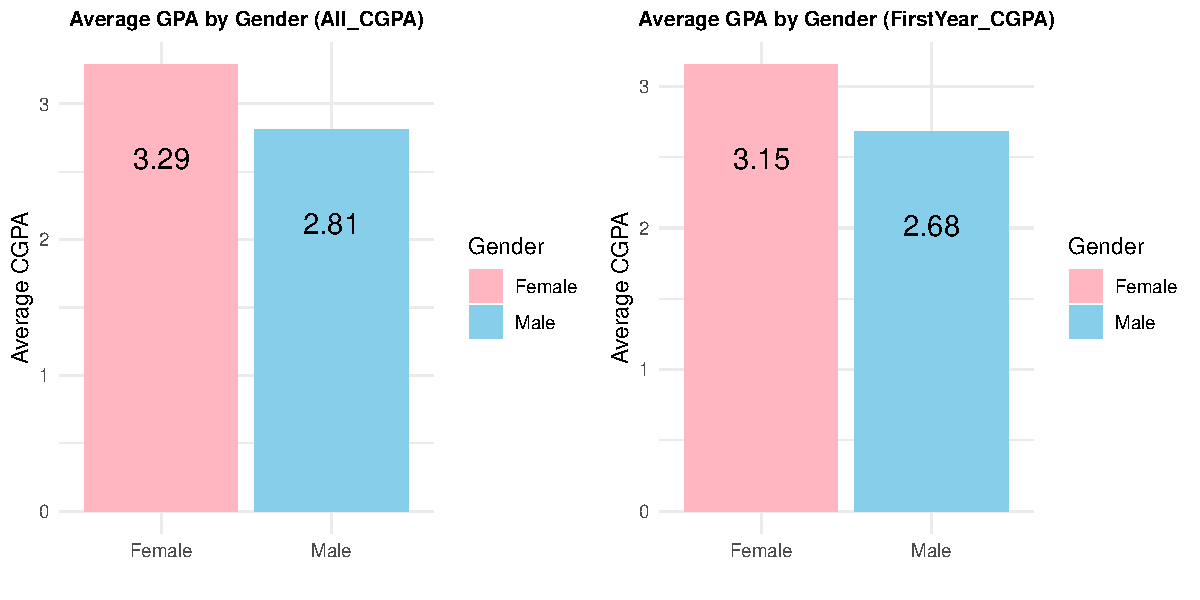
\includegraphics[width=0.9\linewidth]{iesm315_report_files/figure-latex/unnamed-chunk-9-1} \caption{GPA Distribution by Gender}\label{fig:unnamed-chunk-9}
\end{figure}

Fig. 5 compares the average CGPA of students by gender, displayed
separately for two categories: All\_CGPA and FirstYear\_CGPA. Female
students demonstrate higher average GPAs in both categories, with an
average of 3.29 for All\_CGPA and 3.15 for FirstYear\_CGPA. In contrast,
male students achieve averages of 2.81 for All\_CGPA and 2.68 for
FirstYear\_CGPA.

\begin{figure}
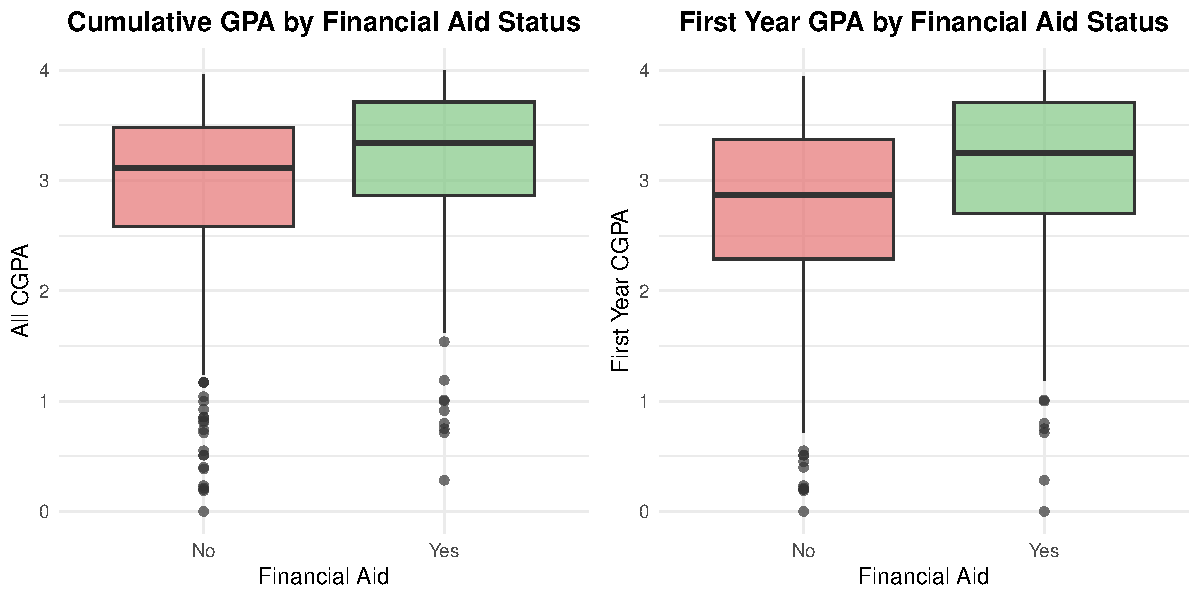
\includegraphics[width=0.8\linewidth]{iesm315_report_files/figure-latex/unnamed-chunk-10-1} \caption{GPA Distribution by Financial Aid Status}\label{fig:unnamed-chunk-10}
\end{figure}

This figure displays the distribution of 1st Year/All Cumulative GPAs
based on whether students received financial aid. The boxplots of both
categories indicates that the median GPA is slightly higher for students
who received financial aid (green) compared to those who did not (red).
The interquartile range (IQR) is similar for both groups, but there are
more outliers in the group without financial aid, particularly on the
lower end of the GPA scale. This suggests that financial aid may provide
a stabilizing effect on academic performance, reducing extreme
variations and potentially supporting better outcomes.

\newpage

\begin{figure}
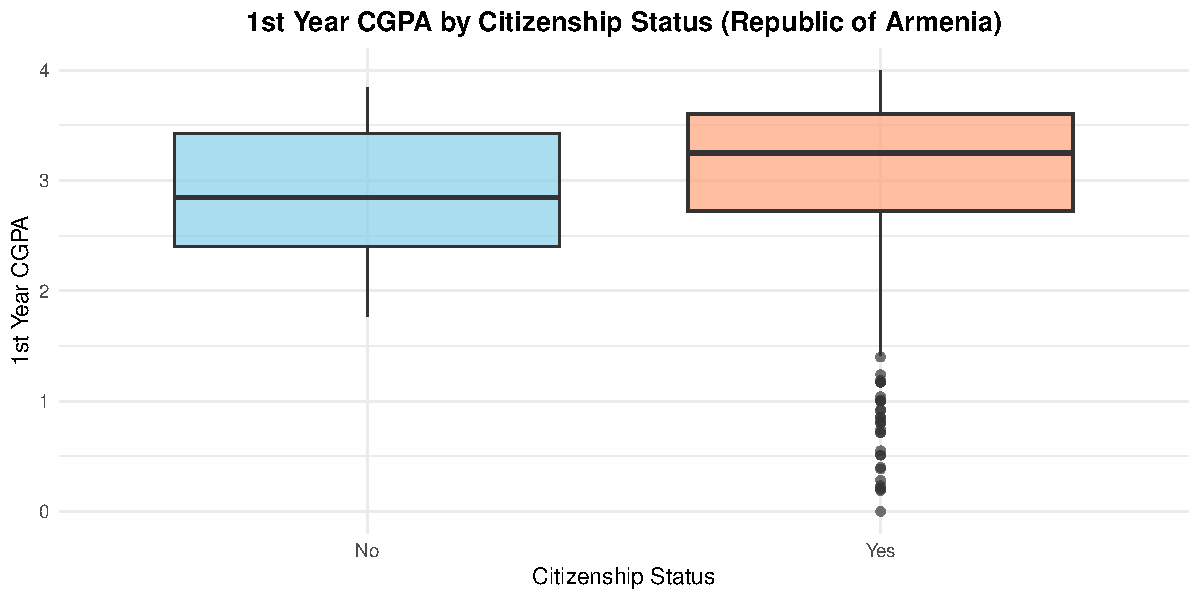
\includegraphics[width=0.9\linewidth]{iesm315_report_files/figure-latex/unnamed-chunk-11-1} \caption{First Year GPA Distribution by RoA Citizenship}\label{fig:unnamed-chunk-11}
\end{figure}

This figure shows boxplots comparing the All CGPA distribution of
students categorized by citizenship status, where ``Yes'' indicates
students with Armenian citizenship, and ``No'' represents non-Armenian
citizens. Students with Armenian citizenship exhibit slightly higher
median GPAs compared to non-Armenian students. The interquartile range
(IQR) for Armenian citizens is broader, while non-Armenian students have
a more compact distribution with fewer outliers.

However, this comparison is inadmissible due to the stark imbalance in
sample sizes: only 26 non-Armenian citizens are included, compared to
1,273 Armenian citizens. Such a significant disparity makes the
comparison unreliable. It would be more appropriate to exclude
non-Armenian citizens from future analyses to avoid skewed
interpretations.

\newpage

\begin{figure}
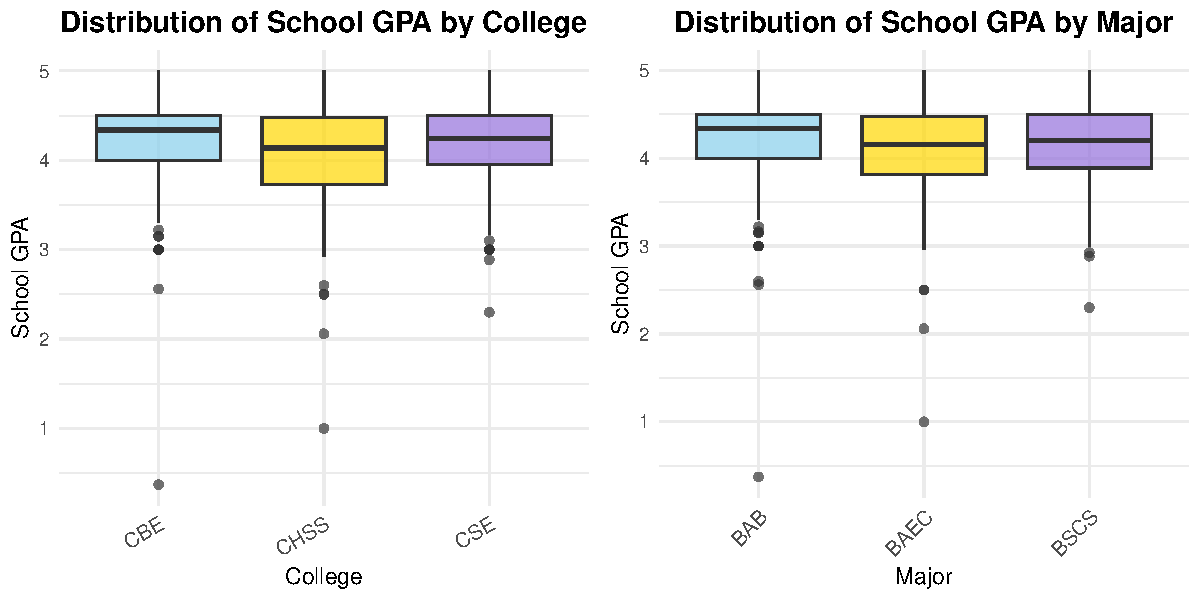
\includegraphics[width=0.9\linewidth]{iesm315_report_files/figure-latex/unnamed-chunk-12-1} \caption{School GPA Distribution by College and Major}\label{fig:unnamed-chunk-12}
\end{figure}

This figure displays the distribution of School\_GPA across colleges
(left) and majors (right). The data is restricted to students enrolled
between 2013 and 2016, as these cohorts had completed their full
cumulative GPA. During this period, there were only three bachelor
programs available: BAB under College CBE, BAEC under CHSS, and BSCS
under CSE.

The boxplots illustrate that the distributions are consistent across
colleges and their corresponding majors, with comparable medians and
interquartile ranges. This indicates limited variability within colleges
but highlights the focus of the dataset on a specific time frame and
program set. The analysis ensures that comparisons remain valid within
the historical context of program availability.

\newpage

\begin{figure}
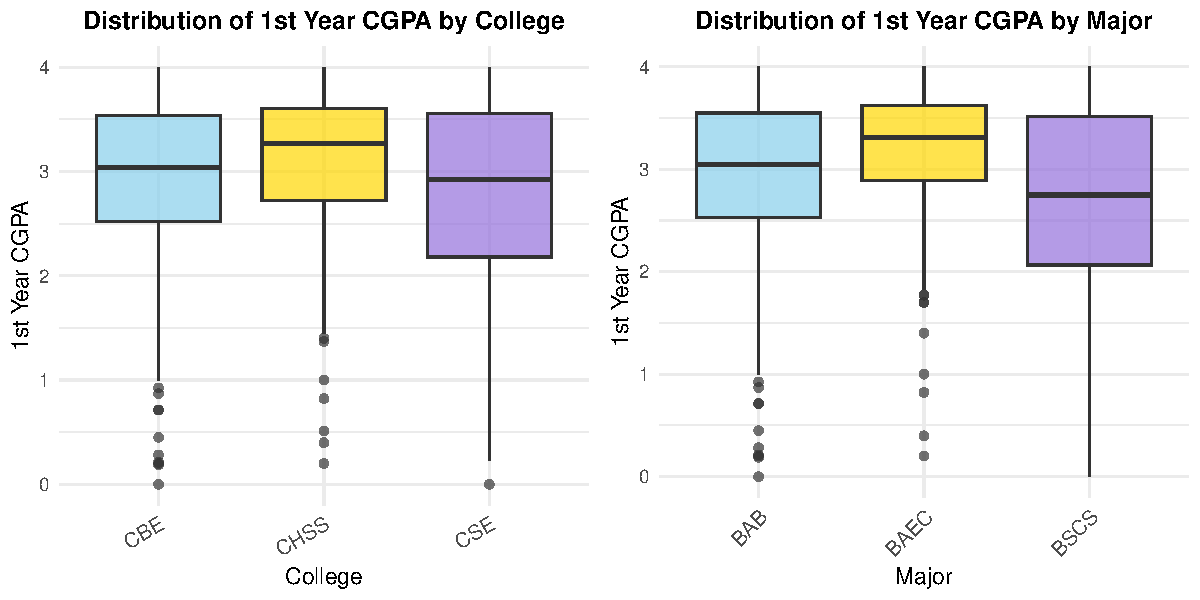
\includegraphics[width=0.9\linewidth]{iesm315_report_files/figure-latex/unnamed-chunk-13-1} \caption{First Year GPA Distribution by College and Major}\label{fig:unnamed-chunk-13}
\end{figure}

A similar figure compares the distribution of 1st Year CGPA across
colleges (left) and majors (right) for students. The data is restricted
to students from the 2013--2016 cohorts, ensuring that the analysis is
aligned with available cumulative GPA data. During this period, three
main undergraduate programs were available: \texttt{BAB} under
\texttt{CBE}, \texttt{BAEC} under \texttt{CHSS}, and \texttt{BSCS} under
\texttt{CSE}.

The distributions across colleges and majors show similar patterns, with
median GPAs being close across all categories. Notably, the College of
Humanities and Social Sciences (CHSS) and its corresponding program
(\texttt{BAEC}) demonstrate slightly higher median GPAs compared to
other colleges and majors. Outliers are present in all categories,
particularly in \texttt{CSE} and \texttt{BSCS}, indicating a broader
variation in student performance for these groups. This comparison
highlights the relative consistency in GPA performance across colleges
and majors while acknowledging differences in variability.

\newpage

\begin{figure}
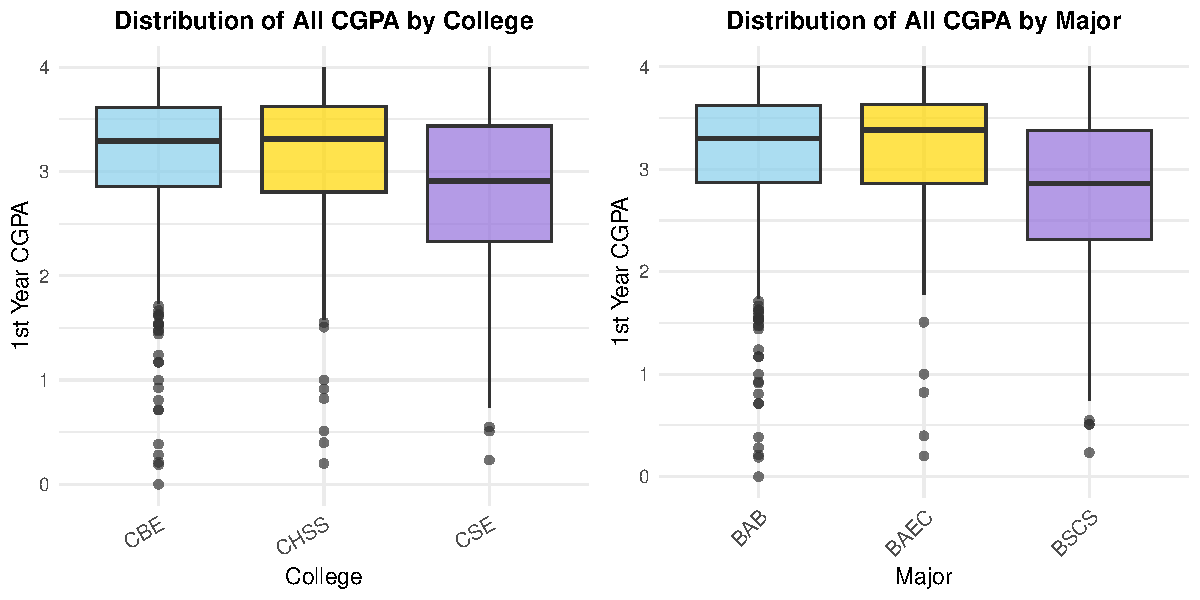
\includegraphics[width=0.9\linewidth]{iesm315_report_files/figure-latex/unnamed-chunk-14-1} \caption{CGPA Distribution by College and Major}\label{fig:unnamed-chunk-14}
\end{figure}

This final figure presents the distribution of \texttt{All\ CGPA} for
students across colleges (left) and majors (right). The distributions
demonstrate similar patterns to the 1st Year CGPA, with slightly higher
median values for \texttt{CHSS} and \texttt{BAEC} compared to the other
colleges and majors.

It is important to note that 1st Year CGPA contributes directly to the
calculation of All CGPA, making this similarity in distribution an
expected behavior. Outliers are present in all categories, reflecting
variations in student performance. This consistency reinforces the role
of early academic performance in shaping cumulative outcomes over the
course of a student's studies.

\newpage

\begin{figure}
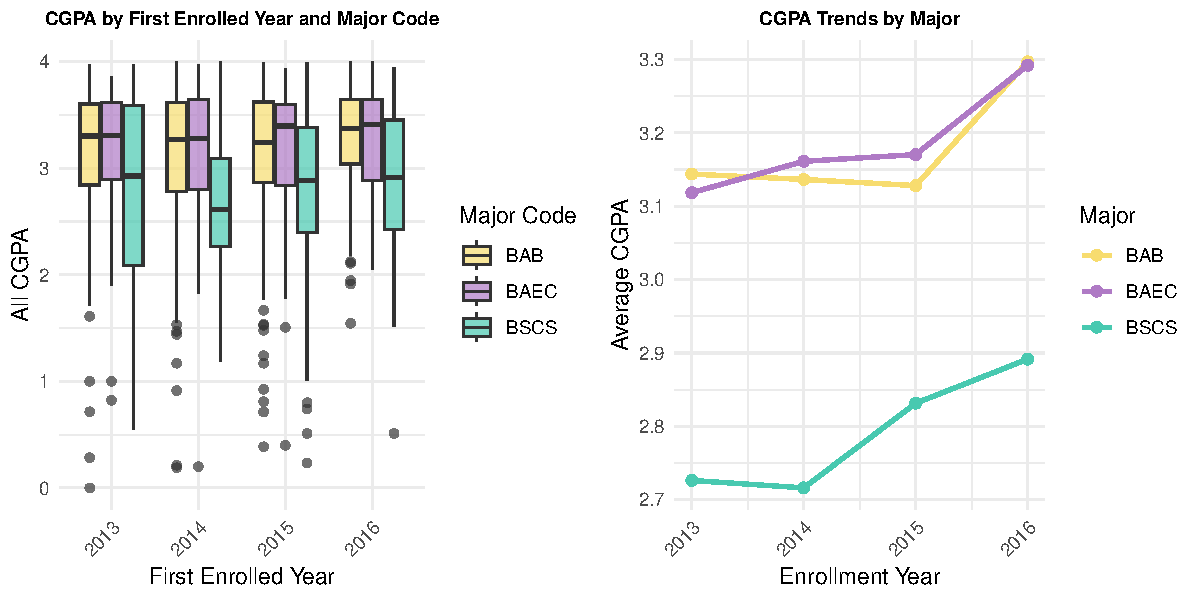
\includegraphics[width=0.9\linewidth]{iesm315_report_files/figure-latex/unnamed-chunk-15-1} \caption{GPA by Enrollment Year and Major}\label{fig:unnamed-chunk-15}
\end{figure}

The left panel shows the distribution of Cumulative GPAs (All CGPA) for
students grouped by their first enrolled year (FirstEnrolled\_Year),
with each boxplot colored by their major code
(FirstEnrolled\_MajorCode). The right panel displays the average
cumulative GPA trends for each major across enrollment years.

The boxplots highlight that BAEC majors generally have higher median
GPAs, while BSCS majors show greater variability and more outliers. The
trend lines reveal that BAEC demonstrates a steady increase in average
GPA, peaking in 2016, whereas BAB remains stable across the years. BSCS,
although initially lower, shows a consistent upward trend, suggesting
improvement over time.

The takeaway is the difference in distributions by Colleges and
Enrollment Year. The latter, however, is relatively niche.

\newpage

\begin{figure}
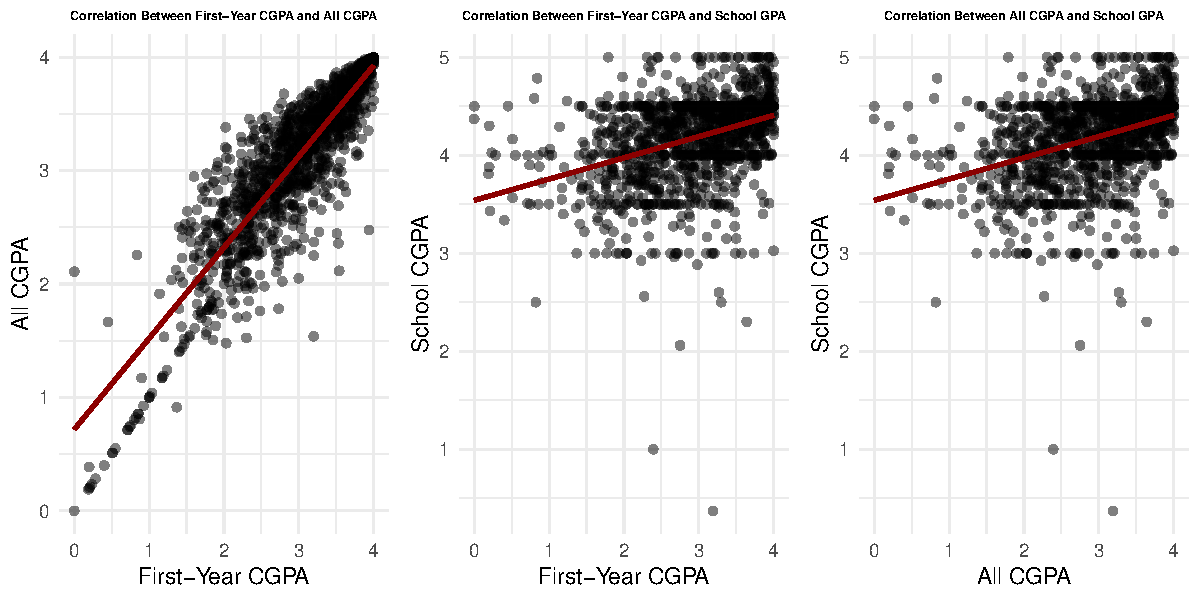
\includegraphics[width=0.9\linewidth]{iesm315_report_files/figure-latex/unnamed-chunk-16-1} \caption{Correlations of GPAs}\label{fig:unnamed-chunk-16}
\end{figure}

The figure displays the correlations between different GPA metrics. The
left panel shows a strong positive correlation between 1st Year CGPA and
All CGPA, which is expected since 1st Year CGPA contributes directly to
the cumulative calculation. The middle panel shows a weaker but
noticeable positive correlation between 1st Year CGPA and School GPA,
highlighting a small association. This is important to consider if both
metrics are included in the analysis, as it may introduce collinearity.
The right panel illustrates a moderate positive correlation between All
CGPA and School GPA, reflecting their cumulative relationship.

Visually, trends are evident, but further numerical analysis is needed
to determine whether the weaker correlation (e.g., between 1st Year CGPA
and School GPA) justifies including both factors in the final analysis.
This step ensures that correlated factors are appropriately managed.

\newpage

\section{Conducting Analysis}\label{conducting-analysis}

\begin{Shaded}
\begin{Highlighting}[]
\CommentTok{\# Correlation between 1st Year GPA and School GPA}
\NormalTok{cor\_test }\OtherTok{\textless{}{-}} \FunctionTok{cor.test}\NormalTok{(gpa\_data}\SpecialCharTok{$}\NormalTok{FirstYear\_CGPA, gpa\_data}\SpecialCharTok{$}\NormalTok{School\_GPA, }
                     \AttributeTok{method =} \StringTok{"pearson"}\NormalTok{)}
\FunctionTok{print}\NormalTok{(cor\_test)}
\end{Highlighting}
\end{Shaded}

\begin{verbatim}
## 
##  Pearson's product-moment correlation
## 
## data:  gpa_data$FirstYear_CGPA and gpa_data$School_GPA
## t = 14.236, df = 1292, p-value < 2.2e-16
## alternative hypothesis: true correlation is not equal to 0
## 95 percent confidence interval:
##  0.3201474 0.4143975
## sample estimates:
##      cor 
## 0.368218
\end{verbatim}

\begin{Shaded}
\begin{Highlighting}[]
\CommentTok{\# Correlation between 1st Year GPA and Overall GPA}
\NormalTok{cor\_test\_uni\_gpa }\OtherTok{\textless{}{-}} \FunctionTok{cor.test}\NormalTok{(gpa\_data}\SpecialCharTok{$}\NormalTok{FirstYear\_CGPA, gpa\_data}\SpecialCharTok{$}\NormalTok{All\_CGPA, }
                            \AttributeTok{method =} \StringTok{"pearson"}\NormalTok{)}
\FunctionTok{print}\NormalTok{(cor\_test\_uni\_gpa)}
\end{Highlighting}
\end{Shaded}

\begin{verbatim}
## 
##  Pearson's product-moment correlation
## 
## data:  gpa_data$FirstYear_CGPA and gpa_data$All_CGPA
## t = 68.054, df = 1300, p-value < 2.2e-16
## alternative hypothesis: true correlation is not equal to 0
## 95 percent confidence interval:
##  0.8711371 0.8950061
## sample estimates:
##       cor 
## 0.8836445
\end{verbatim}

The results reveal a strong positive correlation (0.884) between 1st
Year GPA and Overall GPA, which is expected as the former contributes
directly to the calculation of the latter. On the other hand, the
correlation between 1st Year GPA and School GPA is weaker (0.368) but
still statistically significant.

We previously discussed the visual relationship between 1st Year GPA and
School GPA in the scatterplots, where a weak correlation was observed.
Although the correlation coefficient is below 0.5, indicating a modest
association, we decided to retain both metrics in the analysis. This
decision was made because the correlation is not strong enough to raise
serious concerns about collinearity, but the potential unique
contributions of both factors justify their inclusion for a
comprehensive analysis.

\begin{Shaded}
\begin{Highlighting}[]
\CommentTok{\# Understanding the impact of College on All CGPA with ANOVA}
\NormalTok{oneway\_anova }\OtherTok{\textless{}{-}} \FunctionTok{aov}\NormalTok{(All\_CGPA }\SpecialCharTok{\textasciitilde{}}\NormalTok{ College, }\AttributeTok{data =}\NormalTok{ gpa\_data)}
\FunctionTok{summary}\NormalTok{(oneway\_anova)}
\end{Highlighting}
\end{Shaded}

\begin{verbatim}
##               Df Sum Sq Mean Sq F value   Pr(>F)    
## College        2   22.4  11.209   24.42 3.87e-11 ***
## Residuals   1299  596.2   0.459                     
## ---
## Signif. codes:  0 '***' 0.001 '**' 0.01 '*' 0.05 '.' 0.1 ' ' 1
\end{verbatim}

The ANOVA test confirms that College significantly impacts All CGPA, as
evidenced by the highly significant p-value. This aligns with our
earlier visual observations, where the distribution of GPAs differed
across colleges.

This analysis further reinforces the role of College as a meaningful
factor influencing academic performance. Having established its
importance, we will later proceed to examine the effect of College in
more detail to deepen our understanding of its influence on student
outcomes.

\begin{Shaded}
\begin{Highlighting}[]
\CommentTok{\# Conduct Tukey\textquotesingle{}s test for College}
\NormalTok{tukey\_test }\OtherTok{\textless{}{-}} \FunctionTok{TukeyHSD}\NormalTok{(oneway\_anova)}
\FunctionTok{print}\NormalTok{(tukey\_test)}
\end{Highlighting}
\end{Shaded}

\begin{verbatim}
##   Tukey multiple comparisons of means
##     95% family-wise confidence level
## 
## Fit: aov(formula = All_CGPA ~ College, data = gpa_data)
## 
## $College
##                 diff        lwr         upr     p adj
## CHSS-CBE -0.03637804 -0.1455042  0.07274816 0.7140568
## CSE-CBE  -0.32728750 -0.4389750 -0.21559998 0.0000000
## CSE-CHSS -0.29090946 -0.4226450 -0.15917388 0.0000008
\end{verbatim}

The Tukey test reveals clear differences in performance between
colleges. While there is no significant difference in GPA between CHSS
and CBE, the results indicate that students from CSE perform
significantly worse compared to both CHSS and CBE.

This finding aligns with earlier observations of CSE having lower median
GPAs and greater variability. It highlights the challenges faced by
students in the Computer Science department, where performance
consistently lags behind the other colleges. This analysis reinforces
the need for targeted support or further investigation into the factors
contributing to this disparity.

\begin{Shaded}
\begin{Highlighting}[]
\CommentTok{\# T{-}test for Financial Aid impact on All CGPA}
\NormalTok{t\_test\_finaid }\OtherTok{\textless{}{-}} \FunctionTok{t.test}\NormalTok{(All\_CGPA }\SpecialCharTok{\textasciitilde{}}\NormalTok{ FincialAid\_Received\_AtLeast\_Once, }\AttributeTok{data =}\NormalTok{ gpa\_data)}
\FunctionTok{print}\NormalTok{(t\_test\_finaid)}
\end{Highlighting}
\end{Shaded}

\begin{verbatim}
## 
##  Welch Two Sample t-test
## 
## data:  All_CGPA by FincialAid_Received_AtLeast_Once
## t = -7.0574, df = 1187.1, p-value = 2.878e-12
## alternative hypothesis: true difference in means between group 0 and group 1 is not equal to 0
## 95 percent confidence interval:
##  -0.3430348 -0.1937956
## sample estimates:
## mean in group 0 mean in group 1 
##        2.946075        3.214490
\end{verbatim}

The t-test results indicate a highly significant difference in
cumulative GPA (All CGPA) between students who received financial aid
and those who did not. Specifically, students receiving financial aid
have a significantly higher mean CGPA (3.214) compared to those who did
not (2.946).

The negative confidence interval and t-value further confirm that the
GPA for students without financial aid is consistently lower. This
finding highlights the potential positive impact of financial aid on
student performance, making it a crucial factor in academic success.
This result aligns with previous observations from visualizations and
reinforces the importance of considering financial aid status in the
analysis.

\begin{Shaded}
\begin{Highlighting}[]
\CommentTok{\# T{-}test for gender differences in CGPA}
\NormalTok{t\_test\_gender }\OtherTok{\textless{}{-}} \FunctionTok{t.test}\NormalTok{(All\_CGPA }\SpecialCharTok{\textasciitilde{}}\NormalTok{ Gender, }\AttributeTok{data =}\NormalTok{ gpa\_data)}
\FunctionTok{print}\NormalTok{(t\_test\_gender)}
\end{Highlighting}
\end{Shaded}

\begin{verbatim}
## 
##  Welch Two Sample t-test
## 
## data:  All_CGPA by Gender
## t = 12.241, df = 889.26, p-value < 2.2e-16
## alternative hypothesis: true difference in means between group Female and group Male is not equal to 0
## 95 percent confidence interval:
##  0.3980936 0.5501203
## sample estimates:
## mean in group Female   mean in group Male 
##             3.288330             2.814223
\end{verbatim}

The t-test reveals a significant difference in CGPA based on gender (p
\textless{} 2.2e-16). Female students have a higher mean CGPA (3.288)
than male students (2.814). This significant gender disparity highlights
the potential influence of gender-specific factors on academic
performance, warranting further investigation.

\begin{Shaded}
\begin{Highlighting}[]
\NormalTok{gpa\_data }\OtherTok{\textless{}{-}}\NormalTok{ gpa\_data }\SpecialCharTok{\%\textgreater{}\%}
    \FunctionTok{mutate}\NormalTok{(}\AttributeTok{FirstEnrolled\_Year =} \FunctionTok{as.factor}\NormalTok{(FirstEnrolled\_Year))}

\CommentTok{\# One{-}way ANOVA based on Enrollment Year}
\NormalTok{anova\_year }\OtherTok{\textless{}{-}} \FunctionTok{aov}\NormalTok{(All\_CGPA }\SpecialCharTok{\textasciitilde{}}\NormalTok{ FirstEnrolled\_Year, }\AttributeTok{data =}\NormalTok{ gpa\_data)}
\FunctionTok{summary}\NormalTok{(anova\_year)}
\end{Highlighting}
\end{Shaded}

\begin{verbatim}
##                      Df Sum Sq Mean Sq F value Pr(>F)  
## FirstEnrolled_Year    3    5.1  1.7030   3.603  0.013 *
## Residuals          1298  613.5  0.4726                 
## ---
## Signif. codes:  0 '***' 0.001 '**' 0.01 '*' 0.05 '.' 0.1 ' ' 1
\end{verbatim}

The ANOVA test investigates the influence of enrollment year on
cumulative GPA. The p-value (0.013) indicates a statistically
significant effect of the enrollment year on cumulative GPA. This
suggests slight variations in academic performance based on the year
students enrolled. However, the mean differences across years seem
relatively small, as seen in the exploratory data analysis.

\begin{Shaded}
\begin{Highlighting}[]
\CommentTok{\# Tukey test to find differences between years}
\NormalTok{tukey\_posthoc }\OtherTok{\textless{}{-}} \FunctionTok{TukeyHSD}\NormalTok{(anova\_year)}
\FunctionTok{print}\NormalTok{(tukey\_posthoc)}
\end{Highlighting}
\end{Shaded}

\begin{verbatim}
##   Tukey multiple comparisons of means
##     95% family-wise confidence level
## 
## Fit: aov(formula = All_CGPA ~ FirstEnrolled_Year, data = gpa_data)
## 
## $FirstEnrolled_Year
##                   diff         lwr       upr     p adj
## 2014-2013 -0.023791341 -0.17004899 0.1224663 0.9753353
## 2015-2013 -0.020520559 -0.16526487 0.1242237 0.9834147
## 2016-2013  0.129845549 -0.02221868 0.2819098 0.1247007
## 2015-2014  0.003270782 -0.12557998 0.1321215 0.9999001
## 2016-2014  0.153636890  0.01661451 0.2906593 0.0207766
## 2016-2015  0.150366108  0.01496024 0.2857720 0.0225587
\end{verbatim}

The Tukey post-hoc test further evaluates pairwise differences between
enrollment years. Significant difference is observed between 2016 and
earlier years, with the largest positive difference in GPA for the 2016
cohort (+0.15 compared to 2013) and differences between other pairs
(e.g., 2014-2013, 2015-2014) are not statistically significant as it
could be seen from the graph previously.

\begin{Shaded}
\begin{Highlighting}[]
\CommentTok{\# T{-}test for Financial Aid (0 = No, 1 = Yes)}
\NormalTok{t\_test\_finaid }\OtherTok{\textless{}{-}} \FunctionTok{t.test}\NormalTok{(All\_CGPA }\SpecialCharTok{\textasciitilde{}}\NormalTok{ FincialAid\_Received\_AtLeast\_Once, }\AttributeTok{data =}\NormalTok{ gpa\_data)}
\FunctionTok{print}\NormalTok{(t\_test\_finaid)}
\end{Highlighting}
\end{Shaded}

\begin{verbatim}
## 
##  Welch Two Sample t-test
## 
## data:  All_CGPA by FincialAid_Received_AtLeast_Once
## t = -7.0574, df = 1187.1, p-value = 2.878e-12
## alternative hypothesis: true difference in means between group 0 and group 1 is not equal to 0
## 95 percent confidence interval:
##  -0.3430348 -0.1937956
## sample estimates:
## mean in group 0 mean in group 1 
##        2.946075        3.214490
\end{verbatim}

The Welch Two-Sample T-Test evaluates the relationship between receiving
financial aid and cumulative GPA (CGPA). The results reveal a
significant difference in CGPA between students who received financial
aid and those who did not, with a p-value of less than 2.878e-12. The
mean CGPA for students who received financial aid was 3.214, while for
those who did not, it was 2.946. This finding indicates that financial
aid might contribute positively to academic performance, potentially by
alleviating financial pressures or providing access to necessary
resources. However, additional research is needed to establish the exact
mechanisms driving this relationship.

\begin{Shaded}
\begin{Highlighting}[]
\NormalTok{gpa\_data\_clean }\OtherTok{\textless{}{-}}\NormalTok{ gpa\_data }\SpecialCharTok{\%\textgreater{}\%}
    \FunctionTok{filter}\NormalTok{(}\SpecialCharTok{!}\FunctionTok{is.na}\NormalTok{(FirstYear\_CGPA), }\SpecialCharTok{!}\FunctionTok{is.na}\NormalTok{(College), }\SpecialCharTok{!}\FunctionTok{is.na}\NormalTok{(FirstEnrolled\_MajorCode))}

\NormalTok{anova\_major\_gpa\_college }\OtherTok{\textless{}{-}} \FunctionTok{aov}\NormalTok{(All\_CGPA }\SpecialCharTok{\textasciitilde{}}\NormalTok{ FirstEnrolled\_MajorCode }\SpecialCharTok{*}\NormalTok{ FirstYear\_CGPA }\SpecialCharTok{*}
\NormalTok{    College, }\AttributeTok{data =}\NormalTok{ gpa\_data\_clean)}
\FunctionTok{summary}\NormalTok{(anova\_major\_gpa\_college)}
\end{Highlighting}
\end{Shaded}

\begin{verbatim}
##                                                  Df Sum Sq Mean Sq  F value
## FirstEnrolled_MajorCode                           2   33.0    16.5  171.737
## FirstYear_CGPA                                    1  457.8   457.8 4763.936
## College                                           2    2.5     1.2   12.759
## FirstEnrolled_MajorCode:FirstYear_CGPA            2    0.6     0.3    2.993
## FirstEnrolled_MajorCode:College                   3    0.4     0.1    1.394
## FirstYear_CGPA:College                            2    0.5     0.2    2.467
## FirstEnrolled_MajorCode:FirstYear_CGPA:College    3    0.2     0.1    0.779
## Residuals                                      1286  123.6     0.1         
##                                                  Pr(>F)    
## FirstEnrolled_MajorCode                         < 2e-16 ***
## FirstYear_CGPA                                  < 2e-16 ***
## College                                        3.26e-06 ***
## FirstEnrolled_MajorCode:FirstYear_CGPA           0.0505 .  
## FirstEnrolled_MajorCode:College                  0.2429    
## FirstYear_CGPA:College                           0.0853 .  
## FirstEnrolled_MajorCode:FirstYear_CGPA:College   0.5057    
## Residuals                                                  
## ---
## Signif. codes:  0 '***' 0.001 '**' 0.01 '*' 0.05 '.' 0.1 ' ' 1
\end{verbatim}

The model evaluates how major codes, first-year CGPA, and colleges
collectively influence the cumulative GPA (All\_CGPA). The model reveals
statistically significant effects for the variables
\texttt{FirstEnrolled\_MajorCode} (p \textless{} 2e-16) and
\texttt{FirstYear\_CGPA} (p \textless{} 2e-16), indicating that both the
choice of major and initial academic performance strongly correlate with
final cumulative GPA. However, the interaction effects between
\texttt{FirstEnrolled\_MajorCode}, \texttt{FirstYear\_CGPA}, and
\texttt{College} were not statistically significant, suggesting that
their combined influence does not add further explanatory power beyond
their individual contributions. This indicates that future analyses
could focus on the direct effects of these variables rather than their
interactions.

\subsubsection{Switching}\label{switching}

Switching refers to students transitioning from their initially enrolled
major to a different program. This factor may influence cumulative GPA,
as initial struggles in the original major could impact academic
performance. Although the number of such students is relatively small,
their impact on GPA trends is worth exploring.

\begin{verbatim}
## # A tibble: 6 x 3
##   College Switched Count
##   <chr>      <dbl> <int>
## 1 CBE            0   697
## 2 CBE            1    22
## 3 CHSS           0   275
## 4 CHSS           1    26
## 5 CSE            0   273
## 6 CSE            1     9
\end{verbatim}

\begin{figure}
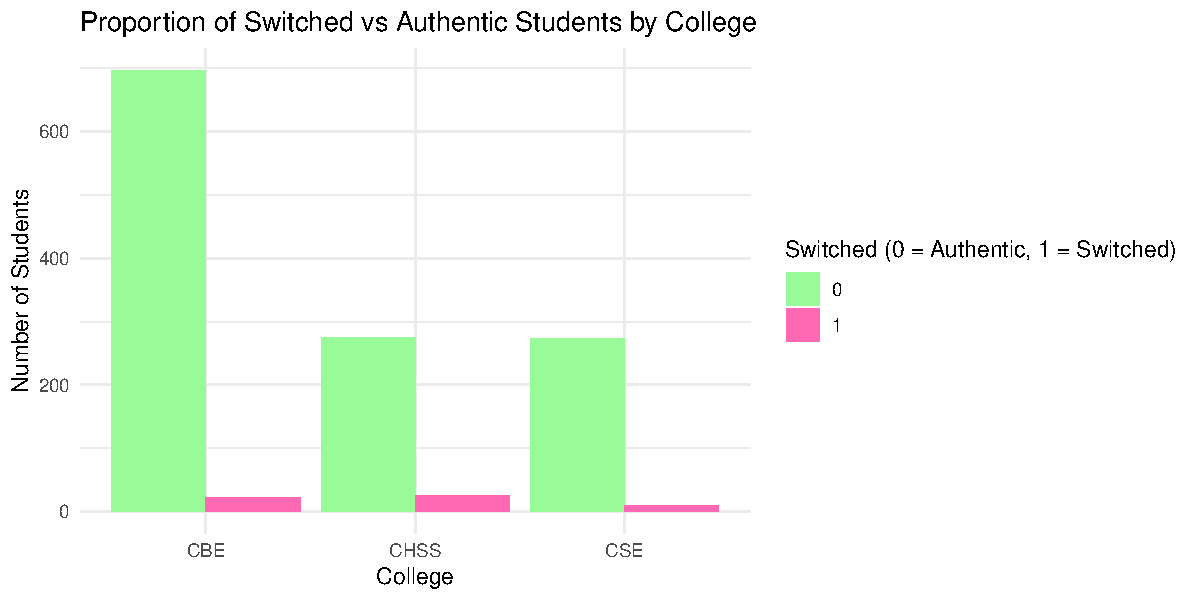
\includegraphics[width=0.9\linewidth]{iesm315_report_files/figure-latex/unnamed-chunk-28-1} \caption{Switched Students by College}\label{fig:unnamed-chunk-28}
\end{figure}

\begin{Shaded}
\begin{Highlighting}[]
\CommentTok{\# T{-}test for CSE}
\NormalTok{t\_test\_cse }\OtherTok{\textless{}{-}} \FunctionTok{t.test}\NormalTok{(All\_CGPA }\SpecialCharTok{\textasciitilde{}}\NormalTok{ Switched, }\AttributeTok{data =}\NormalTok{ combined\_data }\SpecialCharTok{\%\textgreater{}\%}
    \FunctionTok{filter}\NormalTok{(College }\SpecialCharTok{==} \StringTok{"CSE"}\NormalTok{))}
\FunctionTok{print}\NormalTok{(t\_test\_cse)}
\end{Highlighting}
\end{Shaded}

\begin{verbatim}
## 
##  Welch Two Sample t-test
## 
## data:  All_CGPA by Switched
## t = -3.2026, df = 9.2295, p-value = 0.01045
## alternative hypothesis: true difference in means between group 0 and group 1 is not equal to 0
## 95 percent confidence interval:
##  -0.9849688 -0.1713170
## sample estimates:
## mean in group 0 mean in group 1 
##        2.822705        3.400848
\end{verbatim}

For CSE students, a Welch Two Sample t-test revealed that those who
switched programs had significantly higher GPAs compared to those who
stayed, indicating that switching might have helped alleviate
challenges.

\begin{Shaded}
\begin{Highlighting}[]
\CommentTok{\# T{-}test for CBE}
\NormalTok{t\_test\_cbe }\OtherTok{\textless{}{-}} \FunctionTok{t.test}\NormalTok{(All\_CGPA }\SpecialCharTok{\textasciitilde{}}\NormalTok{ Switched, }\AttributeTok{data =}\NormalTok{ combined\_data }\SpecialCharTok{\%\textgreater{}\%}
    \FunctionTok{filter}\NormalTok{(College }\SpecialCharTok{==} \StringTok{"CBE"}\NormalTok{))}
\FunctionTok{print}\NormalTok{(t\_test\_cbe)}
\end{Highlighting}
\end{Shaded}

\begin{verbatim}
## 
##  Welch Two Sample t-test
## 
## data:  All_CGPA by Switched
## t = 4.2961, df = 23.624, p-value = 0.0002561
## alternative hypothesis: true difference in means between group 0 and group 1 is not equal to 0
## 95 percent confidence interval:
##  0.2256250 0.6435214
## sample estimates:
## mean in group 0 mean in group 1 
##        3.181741        2.747168
\end{verbatim}

For CBE students, the t-test also showed significantly higher GPAs for
those who switched, suggesting that transitioning to another program was
beneficial for their academic performance.

\begin{Shaded}
\begin{Highlighting}[]
\CommentTok{\# T{-}test for CHSS}
\NormalTok{t\_test\_chss }\OtherTok{\textless{}{-}} \FunctionTok{t.test}\NormalTok{(All\_CGPA }\SpecialCharTok{\textasciitilde{}}\NormalTok{ Switched, }\AttributeTok{data =}\NormalTok{ combined\_data }\SpecialCharTok{\%\textgreater{}\%}
    \FunctionTok{filter}\NormalTok{(College }\SpecialCharTok{==} \StringTok{"CHSS"}\NormalTok{))}
\FunctionTok{print}\NormalTok{(t\_test\_chss)}
\end{Highlighting}
\end{Shaded}

\begin{verbatim}
## 
##  Welch Two Sample t-test
## 
## data:  All_CGPA by Switched
## t = 4.1908, df = 27.57, p-value = 0.0002578
## alternative hypothesis: true difference in means between group 0 and group 1 is not equal to 0
## 95 percent confidence interval:
##  0.3602288 1.0500357
## sample estimates:
## mean in group 0 mean in group 1 
##        3.192974        2.487842
\end{verbatim}

Similarly, CHSS students who switched programs had significantly higher
GPAs than those who remained, further supporting the idea that switching
can positively impact academic outcomes.

\begin{Shaded}
\begin{Highlighting}[]
\NormalTok{anova\_all\_star\_switched }\OtherTok{\textless{}{-}} \FunctionTok{Anova}\NormalTok{(}\FunctionTok{lm}\NormalTok{(All\_CGPA }\SpecialCharTok{\textasciitilde{}}\NormalTok{ FirstYear\_CGPA }\SpecialCharTok{*}\NormalTok{ Switched }\SpecialCharTok{*}\NormalTok{ College,}
    \AttributeTok{data =}\NormalTok{ combined\_data))}
\FunctionTok{print}\NormalTok{(anova\_all\_star\_switched)}
\end{Highlighting}
\end{Shaded}

\begin{verbatim}
## Anova Table (Type II tests)
## 
## Response: All_CGPA
##                                 Sum Sq   Df   F value    Pr(>F)    
## FirstYear_CGPA                  451.58    1 4701.3154 < 2.2e-16 ***
## Switched                          0.60    1    6.2782  0.012345 *  
## College                           8.94    2   46.5579 < 2.2e-16 ***
## FirstYear_CGPA:Switched           0.08    1    0.8290  0.362721    
## FirstYear_CGPA:College            1.06    2    5.5414  0.004015 ** 
## Switched:College                  0.82    2    4.2720  0.014152 *  
## FirstYear_CGPA:Switched:College   0.83    2    4.3153  0.013555 *  
## Residuals                       123.91 1290                        
## ---
## Signif. codes:  0 '***' 0.001 '**' 0.01 '*' 0.05 '.' 0.1 ' ' 1
\end{verbatim}

In the initial ANOVA test, the analysis evaluates the influence of
first-year CGPA, switching status, and college on cumulative GPA,
including the interactions between these factors. First-year CGPA shows
a highly significant effect on cumulative GPA, which is expected since
it directly contributes to the calculation of the cumulative GPA. The
switching status variable displays marginal significance, suggesting
that changing majors might have a potential, albeit weak, influence on
cumulative GPA. College remains strongly significant, highlighting
notable differences in cumulative GPA based on the college. The
interaction between first-year CGPA and college is significant,
indicating that the impact of first-year performance on cumulative GPA
differs across colleges. However, the interaction between first-year
CGPA and switching is not significant, implying that switching majors
does not notably modify the relationship between first-year GPA and
cumulative GPA.

\begin{Shaded}
\begin{Highlighting}[]
\NormalTok{anova\_all\_star\_switched }\OtherTok{\textless{}{-}} \FunctionTok{Anova}\NormalTok{(}\FunctionTok{lm}\NormalTok{(All\_CGPA }\SpecialCharTok{\textasciitilde{}}\NormalTok{ FirstYear\_CGPA }\SpecialCharTok{*}\NormalTok{ Switched }\SpecialCharTok{*}\NormalTok{ College }\SpecialCharTok{*}
\NormalTok{    FirstEnrolled\_MajorCode, }\AttributeTok{data =}\NormalTok{ combined\_data))}
\FunctionTok{print}\NormalTok{(anova\_all\_star\_switched)}
\end{Highlighting}
\end{Shaded}

\begin{verbatim}
## Anova Table (Type II tests)
## 
## Response: All_CGPA
##                                                         Sum Sq   Df   F value
## FirstYear_CGPA                                          451.38    1 4696.6706
## Switched                                                          0          
## College                                                   0.15    2    0.7683
## FirstEnrolled_MajorCode                                   0.17    2    0.8809
## FirstYear_CGPA:Switched                                           0          
## FirstYear_CGPA:College                                    0.55    2    2.8402
## Switched:College                                                  0          
## FirstYear_CGPA:FirstEnrolled_MajorCode                    0.15    2    0.7757
## Switched:FirstEnrolled_MajorCode                                  0          
## College:FirstEnrolled_MajorCode                                   0          
## FirstYear_CGPA:Switched:College                                   0          
## FirstYear_CGPA:Switched:FirstEnrolled_MajorCode                   0          
## FirstYear_CGPA:College:FirstEnrolled_MajorCode                    0          
## Switched:College:FirstEnrolled_MajorCode                          0          
## FirstYear_CGPA:Switched:College:FirstEnrolled_MajorCode           0          
## Residuals                                               123.59 1286          
##                                                          Pr(>F)    
## FirstYear_CGPA                                          < 2e-16 ***
## Switched                                                           
## College                                                 0.46402    
## FirstEnrolled_MajorCode                                 0.41467    
## FirstYear_CGPA:Switched                                            
## FirstYear_CGPA:College                                  0.05878 .  
## Switched:College                                                   
## FirstYear_CGPA:FirstEnrolled_MajorCode                  0.46058    
## Switched:FirstEnrolled_MajorCode                                   
## College:FirstEnrolled_MajorCode                                    
## FirstYear_CGPA:Switched:College                                    
## FirstYear_CGPA:Switched:FirstEnrolled_MajorCode                    
## FirstYear_CGPA:College:FirstEnrolled_MajorCode                     
## Switched:College:FirstEnrolled_MajorCode                           
## FirstYear_CGPA:Switched:College:FirstEnrolled_MajorCode            
## Residuals                                                          
## ---
## Signif. codes:  0 '***' 0.001 '**' 0.01 '*' 0.05 '.' 0.1 ' ' 1
\end{verbatim}

In the extended ANOVA test, the effect of the first enrolled major is
included, along with its interactions with the other factors. The
addition of this variable helps refine the analysis. While the
first-year CGPA remains significant, switching status loses its marginal
significance when additional variables are considered. College continues
to demonstrate a strong significance, reaffirming its impact on
cumulative GPA. However, the interaction between switching status,
college, and first-year CGPA, which was marginally significant in the
previous test, becomes non-significant after the inclusion of the
enrolled major. This indicates that the major accounts for variability
that switching and college interactions previously explained. Other
significant effects persist, but the diminishing significance of the
interactions highlights how adding new variables can provide clarity on
previously observed effects.

\subsubsection{Final Model}\label{final-model}

\begin{Shaded}
\begin{Highlighting}[]
\NormalTok{lm\_all\_star\_switched }\OtherTok{\textless{}{-}} \FunctionTok{Anova}\NormalTok{(}\FunctionTok{lm}\NormalTok{(All\_CGPA }\SpecialCharTok{\textasciitilde{}}\NormalTok{ FirstYear\_CGPA }\SpecialCharTok{*}\NormalTok{ College }\SpecialCharTok{*}\NormalTok{ FirstEnrolled\_MajorCode }\SpecialCharTok{*}
\NormalTok{    Switched }\SpecialCharTok{+}\NormalTok{ Gender }\SpecialCharTok{+}\NormalTok{ School\_GPA }\SpecialCharTok{+}\NormalTok{ FincialAid\_Received\_AtLeast\_Once, }\AttributeTok{data =}\NormalTok{ combined\_data))}
\FunctionTok{print}\NormalTok{(lm\_all\_star\_switched)}
\end{Highlighting}
\end{Shaded}

\begin{verbatim}
## Anova Table (Type II tests)
## 
## Response: All_CGPA
##                                                         Sum Sq   Df   F value
## FirstYear_CGPA                                          328.51    1 3504.1987
## College                                                   0.08    2    0.4394
## FirstEnrolled_MajorCode                                   0.13    2    0.6710
## Switched                                                          0          
## Gender                                                    2.43    1   25.9547
## School_GPA                                                0.30    1    3.1540
## FincialAid_Received_AtLeast_Once                          0.04    1    0.4380
## FirstYear_CGPA:College                                    0.52    2    2.7838
## FirstYear_CGPA:FirstEnrolled_MajorCode                    0.01    2    0.0418
## College:FirstEnrolled_MajorCode                                   0          
## FirstYear_CGPA:Switched                                           0          
## College:Switched                                                  0          
## FirstEnrolled_MajorCode:Switched                                  0          
## FirstYear_CGPA:College:FirstEnrolled_MajorCode                    0          
## FirstYear_CGPA:College:Switched                                   0          
## FirstYear_CGPA:FirstEnrolled_MajorCode:Switched                   0          
## College:FirstEnrolled_MajorCode:Switched                          0          
## FirstYear_CGPA:College:FirstEnrolled_MajorCode:Switched           0          
## Residuals                                               119.53 1275          
##                                                            Pr(>F)    
## FirstYear_CGPA                                          < 2.2e-16 ***
## College                                                   0.64452    
## FirstEnrolled_MajorCode                                   0.51140    
## Switched                                                             
## Gender                                                  4.022e-07 ***
## School_GPA                                                0.07598 .  
## FincialAid_Received_AtLeast_Once                          0.50821    
## FirstYear_CGPA:College                                    0.06218 .  
## FirstYear_CGPA:FirstEnrolled_MajorCode                    0.95905    
## College:FirstEnrolled_MajorCode                                      
## FirstYear_CGPA:Switched                                              
## College:Switched                                                     
## FirstEnrolled_MajorCode:Switched                                     
## FirstYear_CGPA:College:FirstEnrolled_MajorCode                       
## FirstYear_CGPA:College:Switched                                      
## FirstYear_CGPA:FirstEnrolled_MajorCode:Switched                      
## College:FirstEnrolled_MajorCode:Switched                             
## FirstYear_CGPA:College:FirstEnrolled_MajorCode:Switched              
## Residuals                                                            
## ---
## Signif. codes:  0 '***' 0.001 '**' 0.01 '*' 0.05 '.' 0.1 ' ' 1
\end{verbatim}

In the final model, we combined all hypothesized predictors of
cumulative GPA, including first-year GPA, college, first enrolled major
code, switching behavior, gender, school GPA, and financial aid status.
Interaction terms were added to explore their combined effects on
cumulative GPA. The results show that first-year GPA remains the most
significant factor, as expected, given its direct influence on
cumulative GPA. Gender also demonstrates significance, indicating
differences in performance trends between genders. School GPA is
significant, aligning with our earlier decision to include it despite
its correlation with first-year GPA. However, financial aid status,
while relevant in earlier analyses, does not show significance in this
comprehensive model, suggesting it may be overshadowed by stronger
predictors. Switching behavior and its interactions with college and
major codes provide nuanced insights. These results support the
hypothesis that students who switched majors might have experienced
challenges that impacted their overall performance. Interactions such as
first-year GPA with college and college with first enrolled major code
and switching behavior reveal complex relationships that merit further
investigation. This final model captures the multifaceted nature of
factors influencing cumulative GPA.

\section{Cautions and Results}\label{cautions-and-results}

The analysis faced certain limitations due to restrictions in accessing
complete data provided by OIRA, primarily to safeguard the privacy of
students. Such constraints are not uncommon in real-world research,
where data quality and completeness often pose significant challenges.
It is crucial to fully acknowledge these limitations and ensure that any
interpretations or conclusions drawn from the study remain considerate
of these factors.

In real-life scenarios, dealing with imperfect or incomplete data is a
routine aspect of research. However, what matters is how these
challenges are addressed and accounted for in the analysis. The decision
to limit the scope of testing to a specific set of analyses was made to
maintain focus and clarity, even though other possible tests could have
been conducted to explore additional insights. It is important to
emphasize that this study's results should be examined with an
understanding of the decisions made regarding scope, as well as the
inherent data limitations, to prevent misinterpretation.

\section{Acknowledgements}\label{acknowledgements}

Special thank you to AUA's OIRA for providing the data and our
instructor, Tadamasa Sawada, for guidance throughout this project.

\section{References}\label{references}

\begin{itemize}
\item
  Data provided by AUA's Office of Institutional Research and Assessment
  (OIRA), 2023.
\item
  Liang, Y.-W. (M.), Jones, D., \& Robles-Pina, R. A. (2019). Ethnic and
  gender stereotypes on college students' academic performance.
  Educational Research Quarterly. Retrieved from
  \url{https://www.aabri.com/manuscripts/182858.pdf}
\item
  Marini, J. P., Westrick, P. A., \& Shaw, E. J. (2021). Using SAT®
  scores to inform academic major-related decisions and planning on
  campus. College Board Research. Retrieved from
  \url{https://archive.org/details/ERIC_ED613434}
\item
  Stewart, S., Lim, D. H., \& Kim, J. (2018). Factors influencing
  college persistence for first-time students. Journal of College
  Student Retention: Research, Theory \& Practice. Retrieved from
  \url{https://files.eric.ed.gov/fulltext/EJ1092649.pdf}
\end{itemize}

\end{document}
